\documentclass{exam}
\usepackage[utf8]{inputenc}
\usepackage{pdfpages}
\usepackage{listings}
\usepackage{mathabx}
\graphicspath{}

\date{October 03, 2015}

\begin{document}

\begin{titlepage}
\title{CSC420 Assignment 1}
\author{Monica Li \\
Student Number: 997440899 \\
CDF: gwicked}
\maketitle
\end{titlepage}

\begin{questions}

\question
\begin{parts}
\part Compute convolution of the 2D (grayscale) image and a 2D filter.
\begin{lstlisting}[language=python, frame=single]
def main():
    # create filter
    f = numpy.array([[1,1,1],[1,1,1],[1,1,1]])

    # read image and convolve with filter
    im = imread("image.jpg")
    convolved = convolution(im, f)

def convolution(image, filter):
    # create grayscale image
    img_grey = ( image[...,0] + image[...,1] + image[...,2] ) // 3

    # get size of filter and grayscale image
    f_height, f_width = filter.shape
    o_height, o_width = img_grey.shape

    # padding size: from piazza question, assume odd number dimensions
    # don't need to div by 2 since we're adding to both sides anyway
    h_padding = f_height - 1
    w_padding = f_width - 1

    # get new image with padding
    padded = zeroPad(img_grey, o_height, o_width, h_padding, w_padding)

    # flip filter
    flipped = filter[::-1,::-1]

    # convolve
    img_copy = img_grey.copy()
    for i in range(h):
        for j in range(w):
            img_copy[i][j] = getPixelValue(padded, flipped, i, j)
    return img_copy
	
def zeroPad(img, h, w, h_pad, w_pad):
    # zero matrix
    ni_h = h + h_pad
    ni_w = w + w_pad
    new_img = numpy.zeros((ni_h, ni_w), 'uint8')

    # copy image into matrix
    n = 0
    for i in range(h_pad // 2, ni_h - h_pad // 2):
        m = 0
        for j in range(w_pad // 2, ni_w - w_pad // 2):
            new_img[i][j] = img[n][m]
            m = m + 1
        n = n + 1
	return new_img


def getPixelValue(padded_img, filter, i, j):
    f_h, f_w = filter.shape
    summed = 0
    for k in range(f_h):
        n_j = j
        for l in range(f_w):
            summed = summed + (filter[k][l] * padded_img[i][n_j])
            n_j = n_j + 1
        i = i + 1
	return summed
\end{lstlisting}
 
\part
\begin{subparts}
\subpart Is it possible to write a convolution in one pixel as a dot product between two vectors?
\vspace{5mm}
\begin{flushleft}
Yes, it is possible to write convolution in one pixel as a dot product. You would first flatten the vectors, then dot product them.
\end{flushleft}
\vspace{5mm}
\subpart Is it possible to write the full convolution between the image and the filter via matrix multiplication?
\vspace{5mm}
\begin{flushleft} It is not possible to write full convolution between image and filter via matrix multiplication.
\end{flushleft}
\vspace{5mm}
\end{subparts}
\end{parts}

\question
\begin{parts}
\part
\begin{subparts}
\subpart Given a n x n image, I, and m x m filter, h, what is the computational cost of computing h * I (the convolution)?
\vspace{5mm}
\begin{flushleft}
There are $n^{2}$ pixels and one pixel has $m^{2}$ operations performed. Therefore, the computational cost of computing the convolution is O($n^{2}$ $m^{2}$).
\end{flushleft}
\vspace{5mm}

\subpart What is the computational cost if h is a separable filter?
\vspace{5mm}
\begin{flushleft}
If h is separable, then one filter becomes n x 1 and the other, 1 x n. Each filter's cost is m$n^{2}$. The computational cost if h is separable is O(2m$n^{2}$), simplified to O(m$n^{2}$).
\end{flushleft}
\vspace{5mm}
\end{subparts}

\part  If I first convolve an image with a Gaussian filter with $\sigma$ = 1, and then convolve the output with a Gaussian with $\sigma$ = 2, this gives an equivalent result as if I just convolve the image with a Gaussian with what $\sigma$?
\vspace{5mm}
\begin{flushleft}
Given: $\sigma_1 = 1, \sigma_1 = 1, \sigma_2 = 2$

$\sigma = \sqrt{\sigma_1^{2} + \sigma_1^{2}}
        = \sqrt{1 + 4}
        = \sqrt{5}$
        
An equivalent result is achieved using $\sigma = \sqrt{5}$
\end{flushleft}

\newpage
\part Write a function that creates a Gaussian filter with $\sigma$ as an input parameter.
\begin{lstlisting}[language=matlab, frame=single, breaklines=true]
function out = a1q2c(sigma)
% 2D Gaussian function from Lecture 2: h(u, v) = (1/(pow(2*pi*sigma, 2)))*pow(e, (-(pow(u, 2) + pow(v, 2))/pow(sigma, 2))
% Note: from other sources, the denominator of e's exponent is actually 2*sigma^2, instead of sigma^2 indicated in lecture

% size of filter, assuming default size from imgaussfilt
s = 2*ceil(2*sigma)+1;
filter = zeros(s, s);

% const 1/(2*pi*sigma^2)
const = 1 / (2 * pi * sigma.^2);

% loop through matrix and add values to create gaussian kernel
centre = round(s./2);
for n = 1:s
	for m = 1:s
		exponent = -((n - centre).^2 + (m - centre).^2) / 2*sigma.^2;
		filter(n, m) = const * exp(exponent);
	end
end

out = filter;
end
\end{lstlisting}

\newpage
\part Convolve image.png with a (2D) Gaussian filter with $\sigma$ = 10 and visualize the result (display the result of the convolution).
\begin{lstlisting}[language=matlab, frame=single, breaklines=true]
% create gaussian filter
f10 = fspecial('gaussian', [15 15], 10);

% read and gray image
im = imread('image.jpg');
img = rgb2gray(im);

% using conv2() required doubles, and when using double() the image showed a blank square, so I used imfilter instead, with the argument 'conv' to perform convolution
convolved = imfilter(im, f10, 'conv');
\end{lstlisting}
\begin{figure}[ht]
\caption{Convolved image.png with a 2D Gaussian filter and $\sigma$ = 10}
\centering
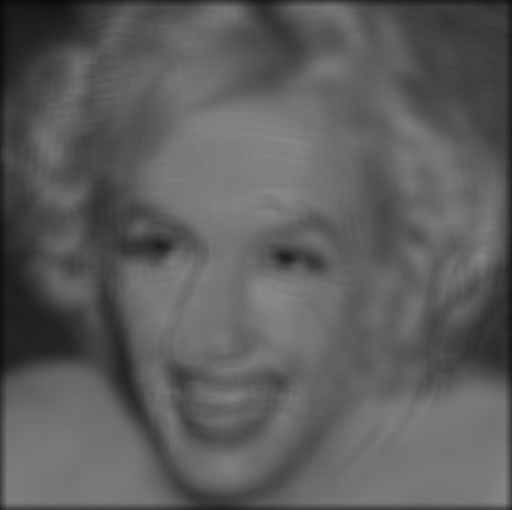
\includegraphics[width=15cm]{a1q2d}
\end{figure}

\part Gaussian filter is separable. How can you use this fact to speed up convolution? What are the vertical and horizontal filters?
\vspace{5mm}
\begin{flushleft}
If the filter matrix is n x m, then when separated, the vertical filter becomes n x 1, and teh horizontal filter becomes 1 x m. Applying two one dimensional filters to the image in succession is faster than applying a single 2D filter, as demonstrated by computation time in Question 2a of this assignment.
\end{flushleft}
\end{parts}

\question
\begin{parts}
\part Compute magnitude of gradients for the attached images waldo.png and template.png.
\begin{lstlisting}[language=matlab, frame=single, breaklines=true]
function out = a1q3a(filename)
% read and gray image
im = imread(filename);
img = rgb2gray(im);

% gradient
g = imgradient(img);

% take max of max for 2D and because sometimes, the values are too small
waldoMaxGradient = g/max(max(g));

out = waldoMaxGradient;
end
\end{lstlisting}
\begin{figure}[ht]
\caption{Computed magnitude of gradients for waldo.png}
\centering
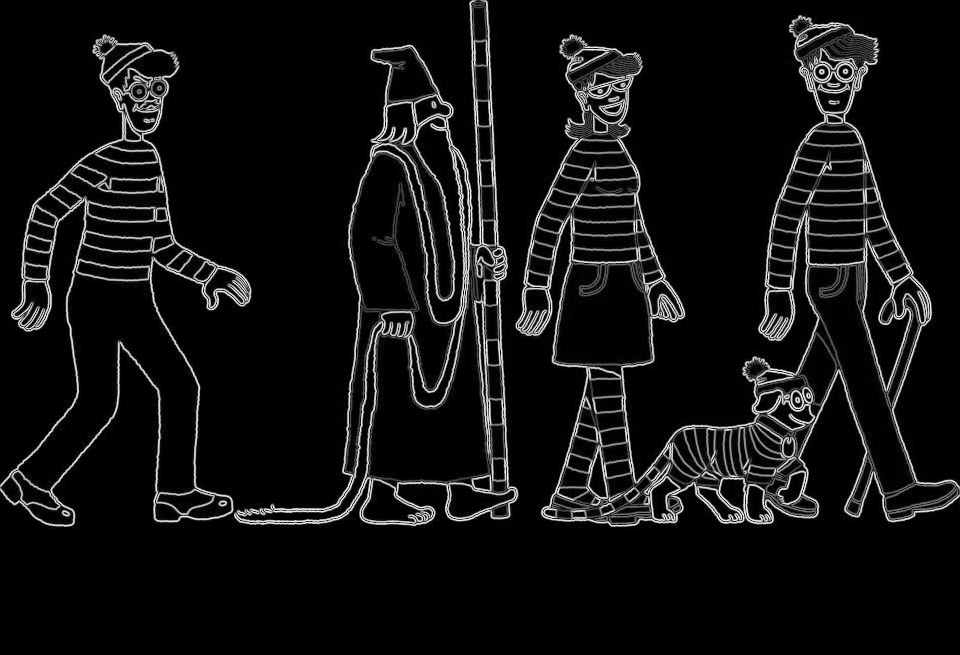
\includegraphics[width=15cm]{a1q3a_waldo}
\end{figure}
\begin{figure}[ht]
\caption{Computed magnitude of gradients for template.png}
\centering
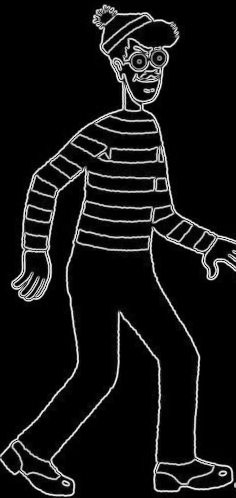
\includegraphics[height=10cm]{a1q3a_template}
\end{figure}

\part Write a function that localizes the template (template.png) in the image waldo.png based on the magnitude of gradients.
\begin{lstlisting}[language=matlab, frame=single, breaklines=true]
% Get max gradients of images, then localise
im = a1q3a('waldo.png');
filter = a1q3a('template.png');
output = a1q3b(im, filter);

% function definition
function out = a1q3b(im, filter)
% normalized cross-correlation
out = normxcorr2(filter, im);

% plot the cross-correlation results
figure('position', [100,100,size(out,2),size(out,1)]);
subplot('position',[0,0,1,1]);
axis off;
axis equal;

% find the peak in response
[y,x] = find(out == max(out(:)));
y = y(1) - size(filter, 1) + 1;
x = x(1) - size(filter, 2) + 1;

% plot the detection's bounding box
figure('position', [300,100,size(im,2),size(im,1)]);
subplot('position',[0,0,1,1]);
axis off;
axis equal;
rectangle('position', [x,y,size(filter,2),size(filter,1)], 'edgecolor', [0.1,0.2,1], 'linewidth', 3.5);
\end{lstlisting}
\begin{figure}[ht]
\caption{Localised template.png on waldo.png}
\centering
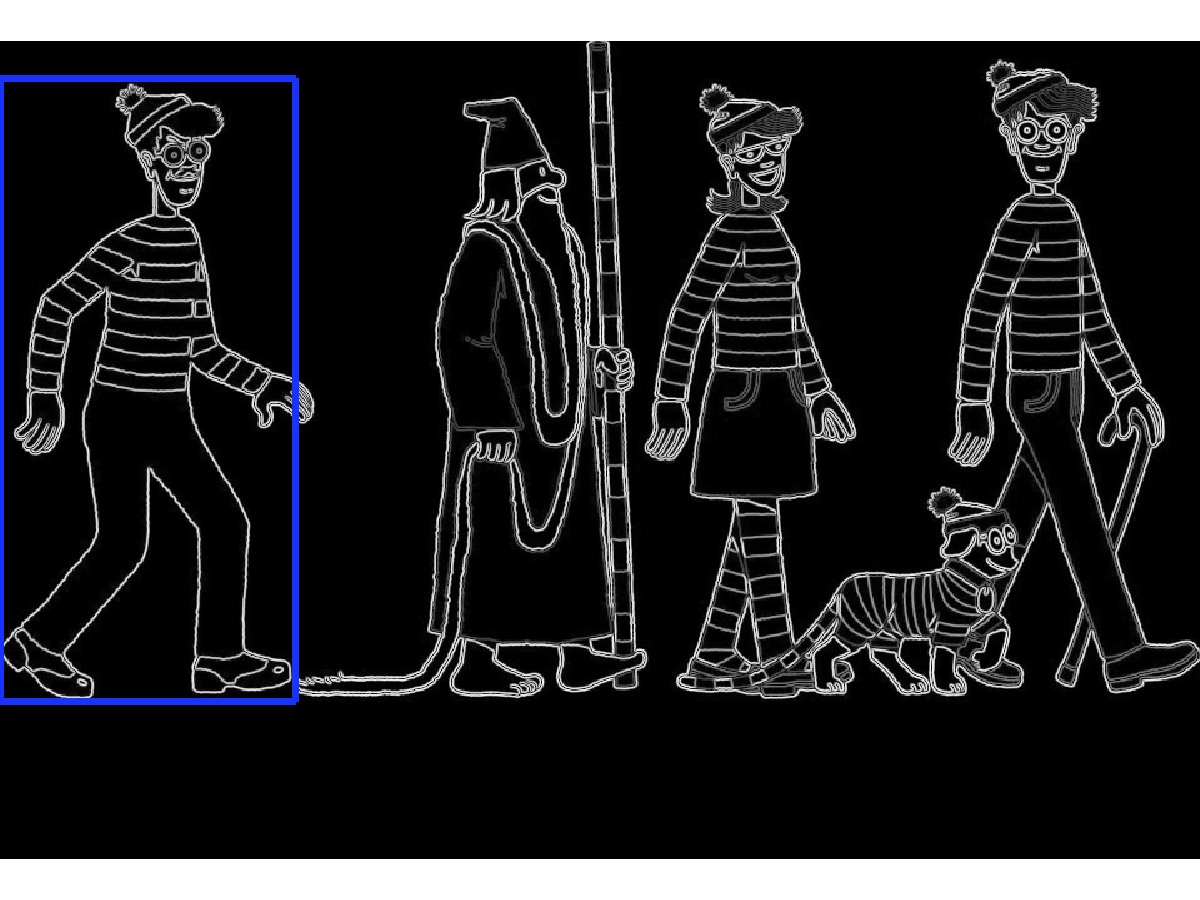
\includegraphics[width=15cm]{a1q3b}
\end{figure}
\end{parts}

\newpage
\question
\begin{parts}
\part Run the Canny edge detector on court.jpg. Play with the parameters so that you get rid of low-contrast edges.
\begin{lstlisting}[language=matlab, frame=single, breaklines=true]
img = a1q3a('court.jpg');
edge(img, 'canny', [0, 0.55];
\end{lstlisting}
\begin{figure}[ht]
\caption{Used Canny edge detector and got read of low-contrast edges}
\centering
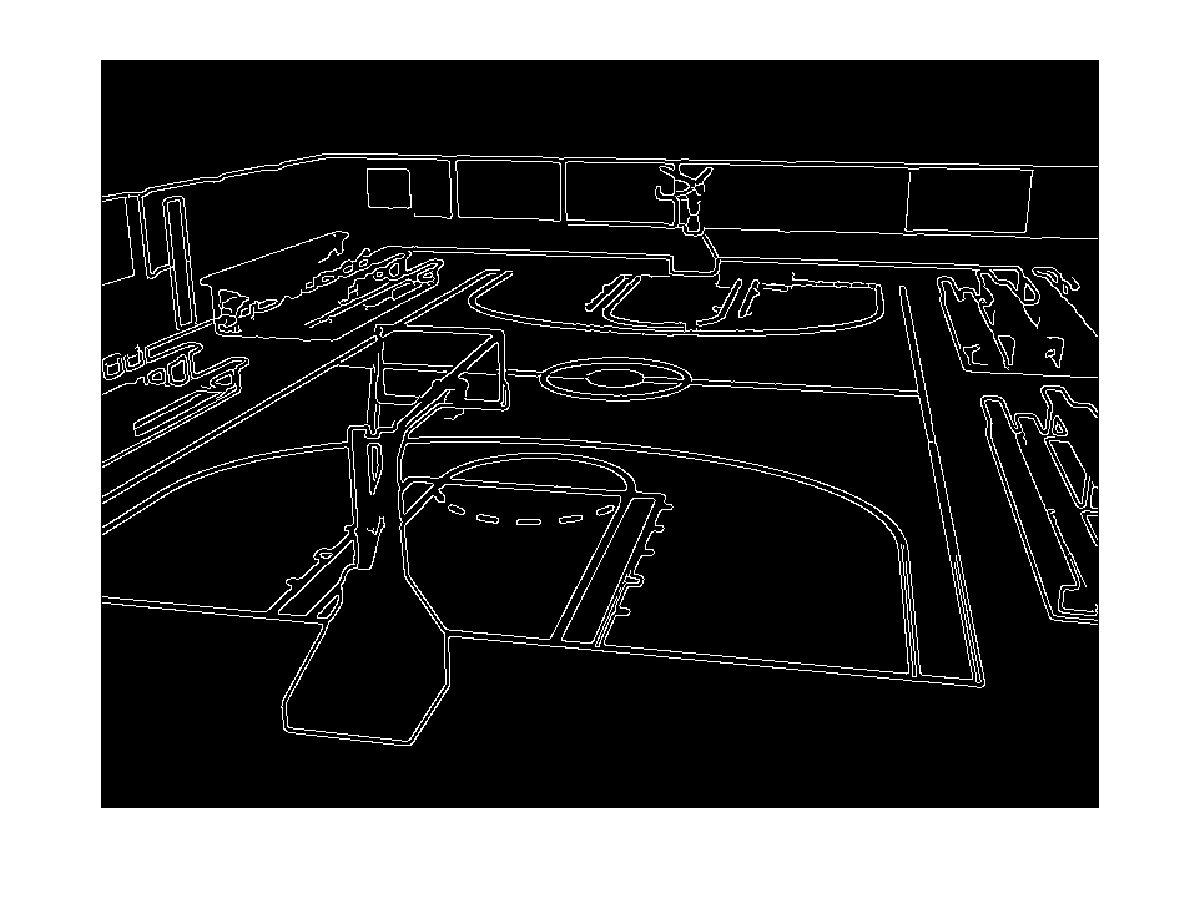
\includegraphics[width=15cm]{a1q4a}
\end{figure}

\part How you could find the bounds of the court in the image?
\vspace{5mm}
\begin{flushleft}
If you already know the image and the direction of one side of the court, find lines that intersect and make a quadrangle.
Alternatively, you could look for corners that make up a large quadrangle in the image.
The court should be made with only four straight lines (this would get rid of other odd shapes, such as those created by outlines of benches, balls, people, etc.).
You can also check to see if your suggested court bounds match up with other models, if you have any.
\end{flushleft}
\end{parts}
\end{questions}

\end{document}
